\documentclass[letterpaper]{article}

%% Language and font encodings
\usepackage[english]{babel}
\usepackage[utf8x]{inputenc}
\usepackage[T1]{fontenc}

%% Sets page size and margins
\usepackage[letterpaper,top=3cm,bottom=2cm,left=3cm,right=3cm,marginparwidth=1.75cm]{geometry}

%% Useful packages
\usepackage{amsmath}
\usepackage{graphicx}
\usepackage[colorinlistoftodos]{todonotes}
\usepackage[colorlinks=true, allcolors=blue]{hyperref}
\usepackage[retainorgcmds]{IEEEtrantools}
\usepackage{amssymb}
\usepackage{natbib}
\usepackage{amsthm}

\title{Constant Elasticity of Substitution Function}
\author{Thiago De Lucena Coelho, Leticia Juarez, Hyok Jung Kim, \and Konstantin Kunze,  Alice Li, Renee S Liu, Curtis Morrill, Zachariah Rutledge, \and Adam Soliman, Hanlin Wei, and Xiurou Wu}

\begin{document}
\maketitle

\begin{abstract}
Your abstract.

\vspace{0.3cm}

\noindent \textbf{Keywords: } Microeconomic theory, consumer theory, production theory, Cobb-Douglas, constant elasticity.

\vspace{0.3cm}

\noindent
\textbf{JEL-Classification: } D11, D21, C61.

\end{abstract}

\pagebreak

\tableofcontents

\pagebreak
\section{Introduction}
Blank
%%%%%%%%%%%%%%%%%%%%%%%%%%%%% INPUT FILE %%%%%%%%%%%%%%%%%%%%%%%%%%%%%

\section{Functional Form}
The CES function is a type of aggregator function which combines two or more types of goods into an aggregate quantity. This aggregator function exhibits constant elasticity of substitution which will be explained later. Before investigating its use in consumer and producer theory, we will observe its functional form and direct properties.
\begin{IEEEeqnarray}{rCl}
    f(x) = \left( \sum_{l=1}^L a_l x_l^{\sigma} \right)^{\frac{1}{\sigma}} \label{eq:CES_base1}
\end{IEEEeqnarray}
$x = (x_1, \cdots, x_L) \in \mathbb{R}_{+}^{L}$. The $\sigma$ determines the level of complementarity among goods. As $\sigma$ increases the level of complementarity also increases.

\subsection{General Characteristics}
\paragraph{Behavior of Derivatives, and Range of Parameters} To characterize the role of parameters $a_l$, and $\sigma$ we need to observe the behavior of $\partial f(x) / \partial x_l$. Partial differentiation of $f(x)$ with respect to $x_l$ gives,
\begin{IEEEeqnarray}{rCl}
    \frac{\partial f(x)}{\partial x_l} & = & a_l x_l^{\sigma-1} f(x)^{1-\sigma} \label{eq:1st_derivative}
\end{IEEEeqnarray}
To insure positivity of first derivative of $f(x)$ with respect to $l$th term, $\partial f(x) / \partial x_l > 0$, we need a condition that $a_l > 0$.

It is common in Economics to assume second derivative of $f(x)$ with respect to $l$th good to be negative. It implies diminishing marginal utility or diminishing marginal product(returns) when applied to consumer or producer theory, respectively. Hence, let us observe the properties of the second derivative of $f(x)$, and figure out appropriate conditions for $\sigma$, and its implications.
\begin{IEEEeqnarray}{rCl}
    \frac{\partial^2 f(x)}{\partial x_l^2} & = & (\sigma-1)a_l x_l^{\sigma-2} f(x)^{1-\sigma} + a_l x^{\sigma-1}(1-\sigma)f(x)^{-\sigma}\frac{\partial f(x)}{\partial x_l} \nonumber \\
    & = & (\sigma-1)a_l x_l^{\sigma-2} f(x)^{1-\sigma} + a_l^2 x^{2\sigma-2}(1-\sigma)f(x)^{1-2\sigma} \nonumber \\
    & = &  (\sigma-1) a_l x_l^{\sigma-2} f(x)^{1-\sigma} \left[1 - a_l \left( \frac{x_l}{f(x)} \right)^{\sigma} \right] \nonumber \\
    && \left( \because a_l x_l^\sigma \leq f(x)^{\sigma} = \sum_{l=1}^L f(x) a_l x_l^{\sigma} \right) \nonumber \\
    & < & 0 \qquad \text{for } -\infty < \sigma < 1, \sigma \neq 0
\end{IEEEeqnarray}
Hence, we can conclude that if $\sigma$ satisfies $-\infty < \sigma < 1$, then CES functional form will exhibit diminishing marginal product (returns) or marginal utility when applied to producer theory or consumer theory respectively. Otherwise it will exhibit increasing marginal product which is used in some special cases.

\paragraph{Homogeneity}
Also, we can easily observe that it is homogeneous of degree one such as,
\begin{IEEEeqnarray}{rCl}
    f(\alpha x) & = & \left( \sum_{l=1}^L a_l (\alpha x_l)^{\sigma} \right)^{\frac{1}{\sigma}} \nonumber \\
    & = & \alpha \left( \sum_{l=1}^L a_l x_l^{\sigma} \right)^{\frac{1}{\sigma}} \nonumber \\
    & = & \alpha f(x)
\end{IEEEeqnarray}

\paragraph{Homotheticity}
When considered as a utility function we can see that CES exhibits homotheticity. Suppose that CES utility function represents a preference relation $\succsim$. Then, we need to show that $x \sim x'$ implies $\alpha x \sim \alpha x'$. We can easily see that $f(x) = f(x')$ implies $f(\alpha x) = f(\alpha x')$ since the function is homogeneous to degree one with respect to $x$.

\paragraph{Monotonicity}
As discussed earlier, if $a_l > 0$ then, for every $l \in \{1, 2,, \cdots L\}$, $\partial f(x) / \partial x_l > 0$ is guaranteed. Moreover since $x \geq x'$ implies $f(x) \geq f(x')$ the function is strictly monotonic when applied to the utility function.

\paragraph{Constant Elasticity of Substitution}
The most important feature of CES function is that its elasticity of substitution is fixed to $\frac{1}{\sigma}$. To show this we compute elasticity of \emph{relative of changes of the $f(x_k) / f(x_l)$} to \emph{relative changes in each two components $x_k / x_l$}.

Demand Function:
	
		\begin{equation}
		\frac{x_k\left(p,m\right)}{x_l\left(p,m\right)} = \frac{\left(\frac{p_k}{\alpha_k}\right)^{\frac{1}{\gamma-1}}}{\left(\frac{p_l}{\alpha_l}\right)^{\frac{1}{\gamma-1}}}
		\end{equation}		
		
		\begin{equation}
		\frac{x_k\left(p,m\right)}{x_l\left(p,m\right)} = \left(\frac{p_k}{p_l}\right)^{\frac{1}{\alpha -1}}\left(\frac{\alpha_l}{\alpha_k}\right)^{\frac{1}{\gamma-1}}
		\end{equation}		

		\begin{equation}
		\ln\left(\frac{x_k\left(p,m\right)}{x_l\left(p,m\right)}\right)= {\frac{1}{\gamma-1}} ln\left(\frac{p_k}{p_l}\right) + {\frac{1}{\gamma-1}} ln\left(\frac{\alpha_l}{\alpha_k}\right)
		\end{equation}		

		\begin{equation}
		\frac{\partial \ln\left(\frac{x_k\left(p,m\right)}{x_l\left(p,m\right)}\right)}{\partial\ln\left(\frac{p_k}{p_l}\right)} = \frac{1}{\gamma-1}
		\end{equation}			

\paragraph{Demand Function}
\begin{IEEEeqnarray}{rCl}
x_k\left(p,w\right) = \frac{\left(\frac{p_k}{\alpha_k}\right)^{\frac{1}{\gamma-1}}w}{\sum_{j=1}^{n} p_j\left(\frac{p_j}{\alpha_j}\right)^{\frac{1}{\gamma-1}}}
\end{IEEEeqnarray}

			
\begin{IEEEeqnarray}{rCl}
\frac{x_k\left(p,w\right)}{x_l\left(p,w\right)}
\nonumber
&=& \frac{\left(\frac{p_k}{\alpha_k}\right)^{\frac{1}{\gamma-1}}w}{\sum_{j=1}^{n} p_j\left(\frac{p_l}{\alpha_l}\right)^{\frac{1}{\gamma-1}}} \times
\frac{\sum_{j=1}^{n} p_j\left(\frac{p_l}{\alpha_l}\right)^{\frac{1}{\gamma-1}}}{\left(\frac{p_l}{\alpha_l}\right)^{\frac{1}{\gamma-1}}w}
\nonumber \\
&=& \frac{\left(\frac{p_k}{\alpha_k}\right)^{\frac{1}{\gamma-1}}}{\left(\frac{p_l}{\alpha_l}\right)^{\frac{1}{\gamma-1}}}
\nonumber \\
&=& \left(\frac{p_k}{p_l}\right)^{\frac{1}{\alpha -1}}\left(\frac{\alpha_l}{\alpha_k}\right)^{\frac{1}{\gamma-1}}
\end{IEEEeqnarray}
		
		
\begin{IEEEeqnarray}{rCl}
\ln\left(\frac{x_k\left(p,w\right)}{x_l\left(p,w\right)}\right)= {\frac{1}{\gamma-1}} ln\left(\frac{p_k}{p_l}\right) + {\frac{1}{\gamma-1}} ln\left(\frac{\alpha_l}{\alpha_k}\right)
\end{IEEEeqnarray}
				
\begin{IEEEeqnarray}{rCl}
\frac{\partial \ln\left(\frac{x_k\left(p,w\right)}{x_l\left(p,w\right)}\right)}{\partial\ln\left(\frac{p_k}{p_l}\right)} = \frac{1}{\gamma-1}
\end{IEEEeqnarray}
	
\paragraph{Cross Differentiation} Let's investigate the characteristics of cross effects, i.e., $\partial^2 f(x) / \partial x_l \partial x_k$.
\begin{IEEEeqnarray}{rCl}
    \frac{\partial^2 f(x)}{\partial x_l \partial x_k} & = & a_l a_k \frac{\sigma}{1-\sigma} x_l^{\sigma-1} x_k^{\sigma-1} f(x)^{-\sigma}
\end{IEEEeqnarray}
We can see that if $\sigma < 1$, then this cross effect is negative. The implication of this property is that if the CES function exhibits the decreasing marginal utility or product, then it also guarantees the negative cross effect.

\subsection{Characteristics of Demand Function}
Its demand function for $k$th good, which will be derived in Section \ref{sec:consumer} is,
\begin{IEEEeqnarray}{rCl}
    x_k(p,w) & = & \frac{w\left( \frac{p_k}{a_k} \right)^{\frac{1}{\sigma-1}}}{\sum_{j=1}^L p_j \left( \frac{p_j}{a_j} \right)^{\frac{1}{\sigma-1}}}
\end{IEEEeqnarray}

\paragraph{Walras' law}
\begin{IEEEeqnarray}{rCl}
    p \cdot x(p, w) &=& p {\frac{\frac{p_{k}}{\alpha_{k}}^{\frac{1}{\sigma-1}}}{\sum_{j=1}^{n} p_{j} \frac{p_{j}}{\alpha_{j}}^{\frac{1}{(\sigma-1)}}}}w  \nonumber \\
	& = & p_{1} \cdot {\frac{\frac{p_{1}}{\alpha_{1}}^{\frac{1}{\sigma-1}}}{\sum_{j=1}^{n} p_{j} \frac{p_{j}}{\alpha_{j}}^{\frac{1}{(\sigma-1)}}}}w + p_{2} \cdot {\frac{\frac{p_{2}}{\alpha_{2}}^{\frac{1}{\sigma-1}}}{\sum_{j=1}^{n} p_{j} \frac{p_{j}}{\alpha_{j}}^{\frac{1}{(\sigma-1)}}}}w + \cdots + p_{L} \cdot {\frac{\frac{p_{L}}{\alpha_{L}}^{\frac{1}{\sigma-1}}}{\sum_{j=1}^{n} p_{j} \frac{p_{j}}{\alpha_{j}}^{\frac{1}{(\sigma-1)}}}}w  \nonumber \\
	& = & {\frac{\sum_{j=1}^{n} wp_{j} \frac{p_{j}}{\alpha_{j}}^{\frac{1}{(\sigma-1)}}}{\sum_{j=1}^{n} p_{j} \frac{p_{j}}{\alpha_{j}}^{\frac{1}{(\sigma-1)}}}} \nonumber \\
	& = &  w
\end{IEEEeqnarray}

\paragraph{Homogeneous of degree zero}
\begin{IEEEeqnarray}{rCl}
	x(\delta p, \delta w) & = & {\frac{\frac{\delta p_{k}}{\alpha_{k}}^{\frac{1}{\sigma-1}}}{\sum_{j=1}^{n} \delta p_{j} \frac{\delta p_{j}}{\alpha_{j}}^{\frac{1}{(\sigma-1)}}}} \cdot \delta w
 \nonumber \\
  & = & {\frac{\frac{ p_{k}}{\alpha_{k}}^{\frac{1}{\sigma-1}}}{\sum_{j=1}^{n} p_{j} \frac{p_{j}}{\alpha_{j}}^{\frac{1}{(\sigma-1)}}}} \cdot w
  \nonumber \\
  & = & x_{k}(p,w)
\end{IEEEeqnarray}

\paragraph{Indirect utility function}
\begin{IEEEeqnarray}{rCl}
    V = \frac{w}{\left(\sum_{j=1}^{n} \alpha_{j}^{\frac{-1}{(\sigma-1)}} p_{j}^{\frac{\sigma}{\sigma-1}}\right)^{\frac{\sigma-1}{\sigma}}}
\end{IEEEeqnarray}
%%%%%%%%%%%%%%%%%%%%%%%%%%%%%%%%%%%%%%%%%%%%%%%%%%%%%%%%%%%%%%%%%%%%% 
%%%%%%%%%%%%%%%%%%%%%%%%%%%%% INPUT FILE %%%%%%%%%%%%%%%%%%%%%%%%%%%%%

\section{Typical Monotone Increasing Transformation}
A typical monotonic increasing transformation for CES functions is applying the natural logarithm to the CES function. Any monotonic transformation of a homothetic function is homothetic. Any monotonic increasing transformation of the CES function would exhibit the same isoquants, and so, the same elasticity of substitution.
	
In the case of CES preference ordering (i.e. demand? utility?), monotonic transformations of the production function do not matter at all.
	
In addition to taking the natural logarithm of the CES function, another monotonic increasing transformation is taking the entire function to the power of $\beta$.{ This results in the "general" form of the utility function as seen in Part 1.}

\subsection{Log version}
Log-CES function, which will be extensively used in Section \ref{sec:special_case}, can be one example of monotone increasing transformation of the CES function.
\begin{IEEEeqnarray}{rCl}
\ln f(x) & = & \frac{1}{\sigma} \ln \left( \sum_{l=1}^L a_l x_l^{\sigma} \right) \label{eq:CES_monotone1}
\end{IEEEeqnarray}
First thing to check is that, does log-transformation change the preference order of variables? To see this we should check if $x \prec x'$ implies $\ln(f(x)) \leq \ln(f(x'))$. This is trivial since log is monotone increasing transformation, so $f(x)) \leq f(x')$ implies $\ln(f(x)) \leq \ln(f(x'))$. The log transformation also satisfies the homotheticity.

\subsection{Scaling of Parameters}
In this section we apply a monotonic increasing transformation $g(\cdot)$ which is defined as $g(x) = x^{\beta}$ where $\beta>0$. Then, applying this monotonic transformation, the CES function can be rewritten as,
\begin{IEEEeqnarray}{rCl}
    \hat{f}(x) = \left( \sum_{l=1}^L a_l x_l^{\sigma} \right)^{\frac{\beta}{\sigma}} \label{eq:CES_monotone2}
\end{IEEEeqnarray}
One big difference made by introducing $\beta$ is that the $\hat{f}(x)$ becomes homogeneous to degree $\beta$ with respect the $x$, that is $\beta\hat{f}{x} = \hat{f}{\beta x}$ since
\begin{IEEEeqnarray}{rCl}
    \hat{f}(\beta x) & = & \left( \sum_{l=1}^L a_l (\beta x_l)^{\sigma} \right)^{\frac{\beta}{\sigma}} \nonumber \\
    & = & \beta^{\frac{\sigma \beta}{\sigma}} \left( \sum_{l=1}^L a_l x_l^{\sigma} \right)^{\frac{\beta}{\sigma}} \nonumber \\
    & = & \beta \left( \sum_{l=1}^L a_l x_l^{\sigma} \right)^{\frac{\beta}{\sigma}} \nonumber \\ 
    & = & \beta \hat{f}(x) \label{eq:CES_monotone2}
\end{IEEEeqnarray}

What happens to the marginal rate of substitution, $\text{MRS}_{jk}$, between $x_j$ and $x_k$? Since,
\begin{IEEEeqnarray}{rCl}
    \frac{\partial \hat{f}(x) / \partial x_j}{\partial \hat{f}(x) / \partial x_k} & = & \frac{\beta \left(\sum_{l=1}^{L}a_l x_l^{\sigma} \right)^{\frac{\beta-\sigma}{\sigma}} a_j x_j^{\sigma-1}}{\beta \left(\sum_{l=1}^{L}a_l x_l^{\sigma} \right)^{\frac{\beta-\sigma}{\sigma}} a_k x_k^{\sigma-1}} \nonumber \\
    & = & \frac{a_j x_j^{\sigma-1}}{a_k x_k^{\sigma-1}} \nonumber \\
    & = & \frac{\partial f(x)/ \partial x_j}{\partial f(x)/ \partial x_k} \nonumber
\end{IEEEeqnarray}
we can see that the marginal rate of substitution is the same before taking the increasing monotone transformation. Since for all $j$, and $k$, this ordinal property of the CES utility function holds, this monotonic transformation do not change the optimal bundle of consumption in the utility maximization problem.

However, since the utility function is no longer homogeneous of degree one, this is cardinal property, and the value function will also be a homogeneous of degree $\beta$.

What happens when $\beta = \sigma$? Then the utility or production function becomes linearly separable with respect to $x$ which makes cross effects zero, $\partial^2 \hat{f}(x) / \partial x_l \partial x_k =0 $. In this case, utility ordering will not depend on the level of individual commodities, that is for $x = (\alpha, x_2, \cdots, x_L)$, and $y = (\alpha, y_2, \cdots, y_L)$, and $x \succ y$, will also imply $x' \succ y'$ where $x' = (\beta, x_2, \cdots, x_L)$, $y' = (\beta, y_2, \cdots, y_L)$, and $\alpha \neq \beta$.
%%%%%%%%%%%%%%%%%%%%%%%%%%%%%%%%%%%%%%%%%%%%%%%%%%%%%%%%%%%%%%%%%%%%% 
\section{Application to consumer theory}
Constant Elasticity of Substitution (CES) functions have been applied extensively to Consumer Theory as seen in our literature review. There are two main reasons why the CES function is so popular in Consumer Theory literature. The first is that its flexibility allows several different relations between goods depending on the value of $\rho$; that is, it is easy to represent perfect compliments (Leontieff shaped utility), perfect substitutes (linear utility), and Cobb-Douglas preferences using the CES utility function. Hence, CES functions are a general case that don't impose too many restrictions on the type of preference the function represents.
\subsection{Characterization in terms of preferences}
The characters of CES function in terms of preference include but are not limit to the following.
\subsubsection{Constant elasticity of substitution}
The first particular characteristic of CES functions that is useful is its constant elasticity of substitution between two goods. That is,\\

$$e_{ij}\left( p,w\right) = - \dfrac{\partial\left[ x_{i}\left( p,w\right)/x_{j}\left( p,w\right) \right] }{\partial\left[ p_{i}/p_{j}\right]} \dfrac{p_{i}/p_{j}}{x_{i}\left( p,w\right)/x_{j}\left( p,w\right)}=\dfrac{1}{1-\sigma}$$

Intuitively, this tells us that the percent increase in relative consumption given a percent change in relative prices will be constant.
Other important characteristics of the CES function include consumers' taste for variety and when the CES function is concave. When we derive these important characteristics, we assume prices are strictly greater than zero, and that the utility function is continuous, differentiable, and locally nonsatiated.
\subsubsection{Taste for variety}
CES preferences imply a taste for variety. To show this, we use a simplified form of CES function and assume symmetry in prices and consumption. The prices of products are given as, $p_1 = \cdots = p_L = p$ and parameters in CES function are all given as unity, that is, $a_1 = \cdots = a_L = 1$. The number of products is given by $L$, so that an increase in $L$ represents the increase in product diversity.

The total expenditure can be represented as
\begin{equation}
I = Lpx.
\end{equation}

Consequently, the demand function can be simplified to,
\begin{equation}
x_{i} = x = \frac{w}{Lp}
\end{equation}

Hence, the indirect utility function can be simplified to,
\begin{equation}
\ln(u) = \ln w + \ln\left(L^{\frac{1-\sigma}{\sigma}}\right) +  \ln\left(p^{\frac{1-\sigma}{\sigma}}\right) \label{eq:variety1}
\end{equation}

Differentiating the indirect utility function \eqref{eq:variety1} gives,

\begin{equation}
\frac{du}{u}  = \left(\frac{1-\sigma}{\sigma}\right) \frac{dL}{L} + \left(\frac{1-\sigma}{\sigma}\right) \frac{dp}{p}
\end{equation}

For simpler notation, define $\hat{x} = \frac{dx}{x}, \hat{u} = \frac{du}{u},\hat{p} = \frac{dp}{p} \text{and } \hat{L} = \frac{dL}{L}$. Then,

\begin{equation}
\hat{u} = \left(\frac{1-\sigma}{\sigma}\right) \hat{L} + \left(\frac{1-\sigma}{\sigma}\right) \hat{p} \label{eq:diversity2}
\end{equation}

From \eqref{eq:diversity2}, we can see that utility increases as variety increases when $\sigma$ is less than 1, and $\sigma \neq 0$ which is in the parameter range for the CES utility function suggested in the earlier sections.
\subsubsection{Concavity of utility function}
Consider a CES utility function with constant returns:

\begin{equation}
u(x_{1},...,x_{n}) = \sum\limits_{l=1}^{L} a_{l} x_{l}^{\sigma}
\end{equation}
This function will be concave if $a_{l}\geq0$ for all $l$ and $\sigma\leq1$. We prove this by first showing that $u$ is quasi-concave. \\
A function is a quasi-concave function if it is a monotone increasing function of a concave function. So let's look for a simple function ``hidden inside'' of $u$.

We note that then
\begin{equation}
u(x)=g(x)^{\frac{1}{\sigma}}
\end{equation}
where
\begin{equation}
g(x)=\sum\limits_{l=1}^{n} a_{l} x_{l}^{\sigma}
\end{equation}

Suppose that $0<\sigma\leq1$. Then we see from Equation 2 that $u(x)$ is a monotone increasing function of $g(x)$. Now it is easy to verify if $0<\sigma\leq1$, then $g(x)$ is concave function, because its Hessian is simply a diagonal matrix with entries of the form:

\begin{equation}
a_{l}\sigma(1-\sigma)x_{l}^{\sigma-2}
\end{equation}

When $0<\sigma\leq1$, this term is non-positive. There $u(x) = g(x)^{\frac{1}{\sigma}}$ is a monotone decreasing fuction of $g(x)$. But if it is a monotone decreasing function of $g(x)$, it is a monotone increasing function of $-g(x)$. Now when $\sigma<0$, the Hessian matrix of $-g(x)$ is a diagonal matrix with entries of the form:

\begin{equation}
-a_{l}\sigma(\sigma-1)x_l^{\sigma-2}
\end{equation}

When $\sigma<0$, these terms are all non-positive and hence $-g$ is a concave function. Then $u(x)$ is a monotone increasing function of $-g(x)$, it must be that $u$ is quasiconcave.

We next show more that $u$ is a concave function. Because $u$ is quasi-concave function that is homogeneous of degree 1, $u$ must also be concave.

We now generalize this for CES functions that are homogeneous of type less than 1. When $u(x)$ is the constant returns to scale function defined, the CES functions that are of degree $k$ less than 1 take the form $u(x)^{k}$ where $0 < k < 1$. Now if we have a concave function $u: \mathbb{R}^{n} \rightarrow \mathbb{R}$, and an increasing concave function $g: \mathbb{R} \rightarrow \mathbb{R}$, then if we define the function $h: \mathbb{R}^n \rightarrow \mathbb{R}$ so that $h(x) = g(u(x))$, then $h$ must be a concave function.

\subsubsection{Completeness}
Preference that generated a CES utility function is complete.
$$\forall x_1, x_2 \in X^L, \quad u(x_1)\geq u(x_2) \quad or \quad u(x_1)\leq u(x_2)$$
$$\therefore x_1 \precsim x_2\quad or \quad x_1 \succsim x_2 $$
\subsubsection{Transitivity}
Preference that generated a CES utility function is transitive.
$$\forall x_1, x_2,x_3 \in X^L, \text{if} \hspace*{2mm} x_1 \succsim x_2 \hspace*{2mm} and \hspace*{2mm} x_2 \succsim x_3$$
$$\quad u(x_1)\geq u(x_2) \quad and \quad u(x_2)\geq u(x_3)$$
$$\therefore u(x_1)\geq u(x_3)$$
$$x_1 \succsim x_3$$
\subsubsection{Monotonicity}
Preference that generated a CES utility function is strongly monotone.
$$\forall x, y \in X^L, \text{if} \hspace*{2mm} x\geq y  \hspace*{2mm} \text{and} \hspace*{2mm} x\neq y$$
$$\text{then}  \hspace*{2mm} x_{i}>y_{i}  \hspace*{2mm}\text{for some} \hspace*{2mm} i  \hspace*{2mm} \text{and} \hspace*{2mm} x_j=y_j  \hspace*{2mm} \text{for}  \hspace*{2mm} j\neq i$$
Let $\Delta x_i = x_i-y_i$
\begin{align*}
u(x) &= \left(\sum_{l=1}^{L}a_lx_l^\sigma\right)^{\dfrac{1}{\sigma}}\\
     &= \left(\sum a_ix_i^\sigma+\sum a_jx_j^\sigma\right)^{\dfrac{1}{\sigma}}\\
     &= \left(\sum a_i(y_i+\Delta x_i)^\sigma+\sum a_jy_j^\sigma\right)^{\dfrac{1}{\sigma}}\\
     &>\left(\sum_{l=1}^{L}a_ly_l^\sigma \right)^{\dfrac{1}{\sigma}} = u(y)
\end{align*}
$$\therefore x\succ y$$
\subsubsection{Convexity}
Preference that generated a CES utility function is strictly convex.
$$\forall x, y,z \in X^L, \text{if} \hspace*{2mm} x\succsim z,  \hspace*{2mm} y\succsim z \hspace*{2mm} \text{and} \hspace*{2mm} x\neq y$$
Let $\alpha \in (0,1)$. $ x\succsim z$ and $y\succsim z$, so $u(x)\geq u(z)$ and $u(y)\geq u(z)$.
\vspace*{1mm}
$$u(\alpha x+(1-\alpha)y)  \hspace*{27mm}$$
\vspace*{-10mm}
\begin{align*}
&= \left(\sum_{l=1}^{L}a_l(\alpha x_l+(1-\alpha)y_l)^\sigma\right)^{\dfrac{1}{\sigma}} \\
& >  \left(\sum_{l=1}^{L}a_l\alpha x_l^\sigma+(1-\alpha)y_l^\sigma\right)^{\dfrac{1}{\sigma}}\\
&= \left(\alpha\sum_{l=1}^{L}a_l x_l^\sigma+(1-\alpha)\sum_{l=1}^{L}a_l y_l^\sigma\right)^{\dfrac{1}{\sigma}}\\
& > \alpha\left(\sum_{l=1}^{L}a_l x_l^\sigma\right)^{\dfrac{1}{\sigma}}+(1-\alpha)\left(\sum_{l=1}^{L}a_l y_l^\sigma\right)^{\dfrac{1}{\sigma}}\\
& \geq \alpha u(z)+(1-\alpha) u(z)\\
&=u(z)
\end{align*}
$$\therefore \alpha x+(1-\alpha)y \succ z$$
\subsubsection{Homotheticity}
Preference that generated a CES utility function is homothetic.
$$\forall x, y \in X^L, \text{if} \hspace*{2mm} x\sim y,  \hspace*{2mm} u(x)=u(y) $$
\begin{align*}
u(tx) =& \left(\sum_{l=1}^{L}a_ltx_l^\sigma\right)^{\dfrac{1}{\sigma}}\\
      =& t\left(\sum_{l=1}^{L}a_lx_l^\sigma\right)^{\dfrac{1}{\sigma}}\\
      =& tu(y)\\
      =&u(ty)
\end{align*}
$$\therefore tx\sim ty$$
\subsection{Constrained optimization}
We derive the demand function under a CES utility function. Our utility maximization problem is,
\begin{IEEEeqnarray}{l}
    \max u = \left( \sum_{l=1}^L a_l x_l^{\sigma} \right)^{\dfrac{1}{\sigma}} \\
    \qquad \text{s.t.} \nonumber \\
    \qquad \qquad \sum_{l=1}^L p_l x_l(p,w) \leq w \nonumber \\
    \qquad \qquad x_l \geq 0, \quad \forall l \in \{1, 2, \cdots, L\}
\end{IEEEeqnarray}
Lagrangian for this problem is,
\begin{IEEEeqnarray}{rCl}
    \mathcal{L} (x,\lambda) & = & \left( \sum_{l=1}^L a_l x_l^{\sigma} \right)^{\frac{1}{\sigma}} + \lambda\left(w - \sum_{l=1}^L p_l x_l\right) + \sum_{l=1}^L \mu_l x_l
\end{IEEEeqnarray}
First order conditions for this problem are,
\begin{IEEEeqnarray}{rCl}
    \frac{\partial \mathcal{L} \left( x, \lambda \right)}{\partial x_j} & = & \left( \sum_{l=1}^L a_l x_l^{\sigma} \right)^{\frac{1-\sigma}{\sigma}}+ a_j x_j^{\sigma-1} - \lambda p_j + \mu_j = 0 \label{eq:foc_j} \\
    \frac{\partial \mathcal{L} (x,\lambda)}{\partial x_k} & = & \left( \sum_{l=1}^L a_l x_l^{\sigma} \right)^{\frac{1-\sigma}{\sigma}} +a_k x_k^{\sigma-1} - \lambda p_k + \mu_k = 0 \label{eq:foc_k} \\
    && \sum_{l=1}^L p_l x_l(p,w) \leq w \nonumber \\
    && \mu_l x_l = 0 \nonumber \\
    && \mu_l \geq 0, x_l \geq 0, \lambda \geq 0 \quad \forall l \in \{1, 2, \cdots, L\} \nonumber
\end{IEEEeqnarray}
If we assume $x_j, x_k > 0$ for any $j$, $k$, and $\mu_j = \mu_k = 0$, then rearranging \eqref{eq:foc_j}, and \eqref{eq:foc_k} gives,
\begin{IEEEeqnarray}{rCl}
    \left( \sum_{l=1}^L a_l x_l^{\sigma} \right)^{\frac{1-\sigma}{\sigma}} \frac{1}{\lambda} & = & \left( \frac{p_j}{a_j} \right) x_l^{1-\sigma} \label{eq:foc_j2} \\
    \left( \sum_{l=1}^L a_l x_l^{\sigma} \right)^{\frac{1-\sigma}{\sigma}} \frac{1}{\lambda} & = & \left( \frac{p_k}{a_k} \right) x_k^{1-\sigma} \label{eq:foc_k2}
\end{IEEEeqnarray}
Equating the righthand side of \eqref{eq:foc_j2} and \eqref{eq:foc_k2} gives,
\begin{IEEEeqnarray}{l}
    x_j^{1-\sigma}\left(\frac{p_j}{a_j}\right) = x_k^{1-\sigma}\left(\frac{p_k}{a_k}\right) \nonumber \\
    \Rightarrow x_j = x_k \left( \frac{p_k}{a_k} \right)^{\frac{1}{1-\sigma}} \left( \frac{p_j}{a_j} \right)^{\frac{-1}{1-\sigma}} \label{eq:foc_comb}
\end{IEEEeqnarray}
Multiplying $p_j$ to both sides of equation \eqref{eq:foc_comb} and summing up over index $j$ gives,
\begin{IEEEeqnarray}{l}
    \sum_{j=1}^L p_j x_j = \sum_{j=1}^L p_j x_k \left( \frac{p_k}{a_k} \right)^{\frac{1}{1-\sigma}} \left( \frac{p_j}{a_j} \right)^{\frac{-1}{1-\sigma}} \nonumber \\
    \Rightarrow w = x_k \left( \frac{p_k}{a_k} \right)^{\frac{1}{1-\sigma}} \sum_{j=1}^L \left( \frac{p_j}{a_j} \right)^{\frac{-1}{1-\sigma}} \label{eq:foc_comb2}
\end{IEEEeqnarray}
Rearranging \eqref{eq:foc_comb2} gives the demand function for $x_k$, which is
\begin{IEEEeqnarray}{rCl}
    x_k & = & \frac{w\left(\frac{p_k}{a_k}\right)^{\frac{1}{\sigma-1}}}{\sum_{j=1}^L p_j \left( \frac{p_j}{a_j}\right)^{\frac{1}{\sigma-1}}} \label{eq:demand}
\end{IEEEeqnarray}

\subsection{Typical manipulations}
\subsubsection{Marginal Rate of Substitution}
The marginal utility for good $x_k$ is
$$MU(x_k) = \dfrac{\partial u(x)}{\partial x_k} = a_kx_k^{\sigma-1}\left(\sum_{l=1}^{L}a_lx_l^\sigma\right)^{\dfrac{1}{\sigma}-1}$$
$$MRS_{kj} = \dfrac{MU(x_k)}{MU(x_j)} = \dfrac{a_k}{a_j}\left( \dfrac{x_k}{x_j} \right)^{\sigma-1} $$
Notice here the marginal utility for good $x_k$ depends on all goods and their parameters. But the marginal rate of substitution for goods $x_k,x_k$ depends only themselves.
\subsubsection{Assumption of $a_l$}
Normally people assume that the sum of $a_l$  equals to one for convenience. Also under this assumption, $a_l$ provides us an insight for the expenditure share of good $x_l$ which we will discuss later.
$$\sum_{l=1}^{L}a_l = 1$$
\subsection{Interpretation in the context of consumption}
Let $p_{l}$ be the price of good $l$.
\subsubsection{Expenditure Share}
Expenditure Share of Good $x_l$:
\begin{equation}
	S_{l} = \dfrac{p_{l}\left(\dfrac{p_{l}}{a_{l}}\right)^{\frac{1}{ \sigma -1}}}{ \sum_{i=1}^L {p_{l}{\left(\dfrac{p_{i} }{a_{l}}\right)^{\frac{1}{ \sigma -1}}}}}
\end{equation}
The expenditure share responds to price change of any good. This also means that when the price of one good $x_l$ changes, the expenditure share of all goods will change.
\subsubsection{Changes of expenditure Share}
Change of the share with respect to price where $S_l = \dfrac{p_lx_l}{w}$:
\begin{equation}
	\frac{\partial{S_{l}}}{\partial{P_{l}}} <0
\end{equation}
When the price of good $x_l$increases, the expenditure share of that good decreases which means consumers switch to goods other than $x_l$

Change of the share with respect to wealth:
\begin{equation}
	\frac{\partial{S_{k}}}{\partial{w}} = 0
\end{equation}
The expenditure share of any good will not respond on wealth level changes.
\subsubsection{Indirect utility function}
Indirect Utility:
\begin{equation}
  	V= U\left(x\left(p_{1},...,p_{L},w\right)\right) = \frac{w}{ \left(\sum_{l=1}^La_{l}^{\frac{\-1}{\sigma-1}}p_{l}\right)^{\frac{\sigma-1}{ \sigma}}}
\end{equation}
Notice here the indirect utility is a homogeneous of degree one with respect to wealth level.
\subsubsection{Relative Demand}
Relative Demand:
\begin{equation}
	\frac{x_{k}}{x_{j}} = \dfrac{\left(\dfrac{p_{k}}{\alpha_{k}}\right)^{\frac{1}{ \sigma -1}}}{\left(\dfrac{ p_{j} }{\alpha_{j}}\right)^{\frac{1}{ \sigma -1}}} = \left(\dfrac{a_jp_{k}}{a_kp_{j}}\right)^{\dfrac{1}{ \sigma -1}} \label{eq:reldemand}
\end{equation}
The relative demand is important here for the reason that we have a constant elasticity of substitution only for the relative demand when there are more than two goods.
\subsubsection{Interpretation of $\sigma$}
$\sigma$ gives us an insight of the elasticity of substitution.
$$e_{ij} = \dfrac{1}{\sigma-1}$$
$$\sigma = \dfrac{e_{ij}+1}{e_{ij}}$$
A higher $\sigma$ means consumers are easily to substitute between goods. When $\sigma \to 1$, goods become perfectly substitutes. When $\sigma \to -\infty$, consumers are hard to substitute between goods which makes them have a Leontief utility function.
\subsubsection{Interpretation of $a$}
$a_l$ is called the share parameter, and we normally we have the assumption that $\sum_{l=1}a_{l}=1$. It also gives us an insight of the marginal utility. Let the marginal utility of good $x_k$ be $MU(x_K)$.
$$MU(x_k) = \dfrac{\partial u(x)}{\partial x_k} = a_kx_k^{\sigma-1}\left(\sum_{l=1}^{L}a_lx_l^\sigma\right)^{\frac{1}{\sigma}-1}$$
So here a larger $a_k$ implies that good $x_k$ has a larger marginal utility
\subsection{Special case of two goods}
The utility maximization problem an representative individual faces is as following, where $0 \neq \sigma \leq 1 $. Here we have goods $x$, $y$ and wealth level $w$. And the prices are denote as $p_x$ and $p_y$ respectively.
\begin{equation}
\begin{array}{rlclcl}
\displaystyle \max_{x,y} & \multicolumn{3}{l}{u(x)=(ax^\sigma+by^\sigma)^{\frac{1}{\sigma}}}\\
\textrm{s.t.} & w=p_{x}x+p_{y}y
\end{array}
\end{equation}

Setting up the Lagrangian
\begin{equation}
\mathcal{L}(x,y,\lambda)=(ax^\sigma+by^\sigma)^{\frac{1}{\sigma}}-\lambda(p_{x}x+p_{y}y-w)
\end{equation}
F.O.C.
\begin{equation}
\frac{\partial \mathcal{L}(x,y,\lambda)}{\partial x} =a(ax^\sigma+by^\sigma)^{\frac{1-\sigma}{\sigma}}x^{\sigma-1}-\lambda p_{x}=0
\end{equation}

\begin{equation}
\frac{\partial \mathcal{L}(x,y,\lambda)}{\partial y} =b(ax^\sigma+by^\sigma)^{\frac{1-\sigma}{\sigma}}b^{\sigma-1}-\lambda p_{y}=0
\end{equation}
\begin{equation}
\frac{\partial \mathcal{L}(x,y,\lambda)}{\partial \lambda} =-(p_{x}x+p_{y}y-w)=0
\end{equation}

Combining first and second equations above,
\begin{equation}
\frac{x}{y} =(\frac{bp_{x}}{ap_{y}})^{\dfrac{1}{\sigma-1}} \Rightarrow x= (\frac{bp_{x}}{ap_{y}})^{\frac{1}{\sigma-1}}y
\end{equation}
Plug this into the budget constraint equation
\begin{equation}
x=\frac{w(bp_{x})^{\frac{1}{\sigma-1}}}{b^{\frac{1}{\sigma-1}}p_{x}^{\frac{\sigma}{\sigma-1}}+a^{\frac{1}{\sigma-1}}p_{y}^{\frac{\sigma}{\sigma-1}}}
\end{equation}

\begin{equation}
y=\frac{w(ap_{y})^{\frac{1}{\sigma-1}}}{b^{\frac{1}{\sigma-1}}p_{x}^{\frac{\sigma}{\sigma-1}}+a^{\frac{1}{\sigma-1}}p_{y}^{\frac{\sigma}{\sigma-1}}}
\end{equation}
Therefore, the constant elasticity of substitution could be derived
\begin{equation}
\frac{x}{y}=(\frac{p_{x}}{p_{y}}\frac{b}{a})^{\frac{1}{\sigma-1}} \Rightarrow ln\frac{x}{y}=\frac{1}{\sigma-1}ln\frac{p_{x}}{p_{y}}+\frac{1}{\sigma-1}ln\frac{b}{a} \Rightarrow \frac{d ln\frac{x}{y} }{ d ln\frac{p_{x}}{p_{y}}}=\frac{1}{\sigma-1}
\end{equation}
The indirect utility function is

\begin{equation}
v(p_{x},p_{y},w)=\frac{w}{(a^{-\frac{1}{\sigma-1}}p_{x}^{\frac{\sigma}{\sigma-1}}+b^{-\frac{1}{\sigma-1}}p_{y}^{\frac{\sigma}{\sigma-1}})^{\frac{\sigma-1}{\sigma}}}
\end{equation}

The preference relationship represented by CES utility function is homothetic, the indifference curves have the same slope at $(x,y)$ and at $(tx,ty)$ for any $t > 0$. The indifference curves below are drawn based on the CES utility function $u(x,y)=(3x^{0.5}+4y^{0.5})^2$. We draw four indifference curves under utility level at 15, 18, 20 and 22.
\begin{center}
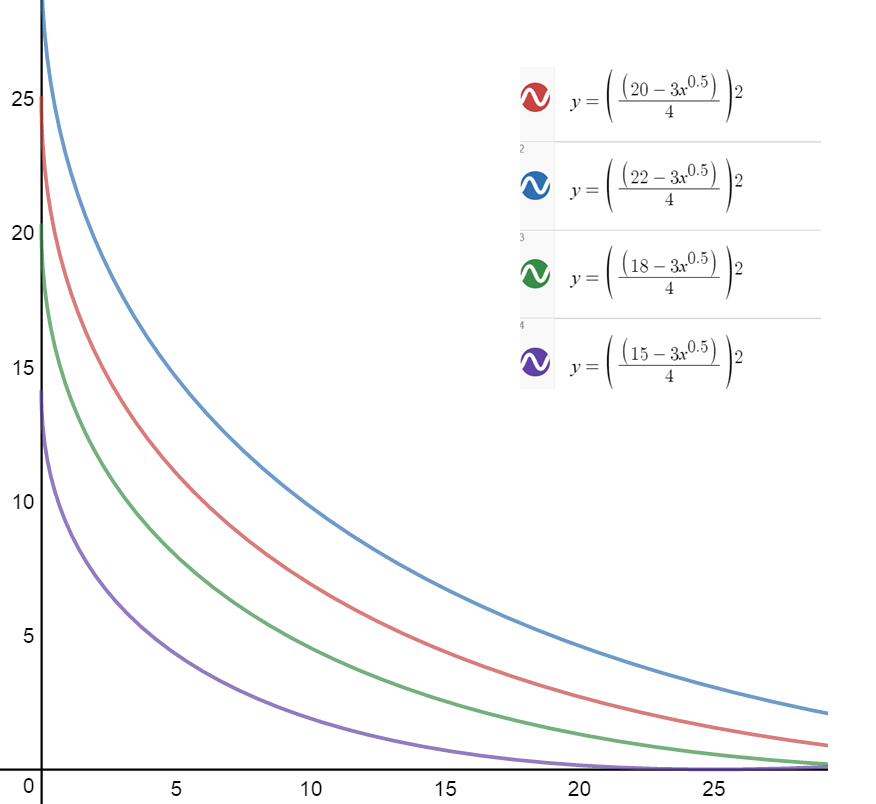
\includegraphics[width=13cm]{Untitled.png}
\end{center}

%%%%%%%%%%%%%%%%%%%%%%%%%%%%%%%%%%%%%%%%%%%%%%%%%%%%%%%%%%%%%%%%%%%%%%%
\section{Application to Production Theory}
\subsection{The General Problem}
Production theory is based on the notion that firms want minimize the costs of inputs needed to produce a certain amount of output.  This problem can be presented as a constrained minimization problem where the objective function is the input cost function and the constraint is the CES production function. Specifically, this problem can be represented as follows:

\begin{equation*}
\begin{aligned}
& \underset{x_1, x2, \cdots , x_L}{\text{minimize}}
& & \sum_{l=1}^L p_ix_i \\
& \text{subject to}
& & q = \bigg( \sum_{l=1}^L a_ix_i^\sigma \bigg) ^{\frac{1}{\sigma}}
\end{aligned}
\end{equation*}

Where $p_i$ is the price of input i, $x_i$ is the amount of input i used in production, $a_i$ is the share of input i used in production and $\sum_{i=1}^L = 1$, q is the amount of output produced by the firm, and $\frac{1}{1- \sigma}$ is the elasticity of substitution between inputs i and j. From this, we can set up a Lagrangian function as follows:

\begin{equation*}
\mathcal{L}(x_1, x_2, \cdots , x_L , a_1, a_2, \cdots, a_L, \lambda) =\sum_{l=1}^L p_ix_i  + \lambda  \bigg[ q - \bigg( \sum_{l=1}^L a_ix_i^\sigma \bigg) ^{\frac{1}{\sigma}} \bigg]
\end{equation*}
In order to solve for the optimal input levels $(x_1, x_2, \cdots, x_L)$, we need to look at the first order conditions of the Lagrangian and solve for $x_{\ell}$.

The first order conditions can be expressed as follows:
\begin{equation*}
\begin{aligned}
& \frac{\partial \mathcal{L}}{\partial x_1} = p_1 + \lambda \bigg[\Big(\sum_{i=1}^L a_1X_1^\sigma \Big)^\frac{1-\sigma}{\sigma}a_ix_i^{\sigma - 1} \bigg] &= 0  \\
& \qquad\vdots \\
& \frac{\partial \mathcal{L}}{\partial x_{L}} = p_L + \lambda \bigg[\Big(\sum_{i=1}^L a_iX_i^\sigma \Big)^\frac{1 - \sigma}{\sigma} a_Lx_L^{\sigma - 1}\bigg] &= 0
\end{aligned}
\end{equation*}

From this we get:
\begin{equation*}
\begin{aligned}
& p_1 &= - \lambda \bigg[\Big(\sum_{i=1}^L a_1X_1^\sigma \Big)^\frac{1-\sigma}{\sigma}a_ix_i^{\sigma - 1} \bigg] \\
& \qquad \vdots \\
& p_L &= - \lambda \bigg[\Big(\sum_{i=1}^L a_LX_L^\sigma \Big)^\frac{1-\sigma}{\sigma}a_ix_i^{\sigma - 1} \bigg]
\end{aligned}
\end{equation*}

By using $\frac{\frac{\partial \mathcal{L}}{\partial x_i}}{\frac{\partial \mathcal{L}}{\partial x_{\ell}}}$, we can derive an expression for $x_i$ in terms of $x_{\ell}$.
\begin{equation*}
x_i = \bigg[\Big(P_ia_{\ell} \Big)^{\frac{\sigma}{\sigma - 1}} \Big(P_{\ell}a_i \Big)^{\frac{-\sigma}{\sigma - 1}} \bigg]x_{\ell}
\end{equation*}
Note that each $x_i$ can be expressed in terms of $a_i, P_i, \sigma, and x_{\ell}$.  By taking each expression for $x_i$ to the power of $\sigma$ and plugging them into the constraint, we get the following expression expression:
\begin{equation*}
q = a_{\ell}x_{\ell} + a_2\Big(P_ia_{\ell} \Big)^{\frac{\sigma}{\sigma - 1}} \Big(P_{\ell}a_i \Big)^{\frac{-\sigma}{\sigma - 1}} + \cdots + a_L\Big(P_ia_{\ell} \Big)^{\frac{\sigma}{\sigma - 1}} \Big(P_{\ell}a_i \Big)^{\frac{-\sigma}{\sigma - 1}} \iff
\end{equation*}
\begin{equation*}
x_{\ell}^{*}(q, a_1, \cdots, a_L, P_1, \cdots, P_L) = \frac{q}{\bigg[a_{\ell} + \Big[\sum_{i \neq \ell} a_i  \Big(\frac{P_i}{a_i} \Big)^{\frac{\sigma}{\sigma - 1}} \Big] \Big(\frac{P_{\ell}}{a_{\ell}} \Big)^{\frac{-\sigma}{\sigma - 1}} \bigg]^{\frac{1}{\sigma}}}  \implies
\end{equation*}
\begin{equation*}
x_{\ell}^{*} (q, a_1, \cdots, a_L, P_1, \cdots, P_L) = \frac{q \Big( \frac{P_{\ell}}{a_{\ell}} \Big)^{\frac{1}{\sigma - 1}}}{\bigg[\sum_{i=i}^L a_i \Big(\frac{P_i}{a_i}\Big)^\frac{\sigma}{\sigma-1} \bigg]^\frac{1}{\sigma}}
\end{equation*}
And thus the optimal input levels can be determined by the amount of output (q) the firm wishes to produce, the share of the inputs $(a_i)$, the prices of the inputs $(P_i)$, and the parameter value $\sigma$.

\subsection{Homogeneity of the CES Production Function}
The CES production function described by $\bigg( \sum_{l=1}^L a_ix_i^\sigma \bigg) ^{\frac{k}{\sigma}}$ is homogeneous of degree k. [ENTER DERIVATION HERE] \\

\subsection{Homogeneity of the Input Demand Functions Derived from the CES Production Function}
\subsubsection{Homogeneity of Degree 1 in Output}
Clearly we can see that the input demand function is homogeneous of degree 1 in output.  This can be seen by the following example. For all $\alpha > 0$:
\begin{equation*}
x_{\ell}^{*}(\alpha q, a_1, \cdots, a_L, P_1, \cdots, P_L) = \frac{\alpha q}{\bigg[a_{\ell} + \Big[\sum_{i \neq \ell} a_i  \Big(\frac{P_i}{a_i} \Big)^{\frac{\sigma}{\sigma - 1}} \Big] \Big(\frac{P_{\ell}}{a_{\ell}} \Big)^{\frac{-\sigma}{\sigma - 1}} \bigg]^{\frac{1}{\sigma}}} = \alpha x_{\ell}^{*}(q, a_1, \cdots, a_L, P_1, \cdots, P_L)
\end{equation*}
\subsubsection{Homogeneity of Degree Zero in Prices and Input Shares}
In addition, we can see that the input demand function is also homogeneous of degree zero in prices.  This can be seen by the following for all $\alpha >0$:
\begin{equation*}
\begin{aligned}
&x_{\ell}^{*}(q, a_1, \cdots, a_L, \alpha P_1, \cdots, \alpha P_L) &= \frac{q \Big( \frac{\alpha P_{\ell}}{a_{\ell}} \Big)^{\frac{1}{\sigma - 1}}}{\bigg[\sum_{i=i}^L a_i \Big(\frac{\alpha P_i}{a_i}\Big)^\frac{\sigma}{\sigma-1} \bigg]^\frac{1}{\sigma}} \\
& &= \frac{\alpha^{\frac{1}{\sigma - 1}}q \Big( \frac{P_{\ell}}{a_{\ell}} \Big)^{\frac{1}{\sigma - 1}}}{\alpha^{\frac{1}{\sigma - 1}}\bigg[\sum_{i=i}^L a_i \Big(\frac{P_i}{a_i}\Big)^\frac{\sigma}{\sigma-1} \bigg]^\frac{1}{\sigma}} \\
& &= x_{\ell}^{*}(q, a_1, \cdots, a_L, P_1, \cdots, P_L) \\
\end{aligned}
\end{equation*}
[ADD DERIVATION OF HOMOGENEITY OF DEGREE 0 IN INPUT SHARES HERE]
%%%%%%%%%%%%%%%%%%%%%%%%%%%%%%%%%%%%%%%%%%%%%%%%%%%%%%%%%%%%%%%%%%%%%%%
\section{Important Special Cases} \label{sec:special_case}
\subsection{Cobb-Douglas: When $\sigma$ Tend to Zero}
When $\sigma \rightarrow 0$, then the utility function in \eqref{eq:utility} becomes Cobb-Douglas utility function. To show this, first take natural logarithm on \eqref{eq:utility}.
\begin{IEEEeqnarray}{rCl}
    \ln u = \frac{\ln(\sum_{l=1}^L a_l x_l^{\sigma})}{\sigma} \label{eq:lnu}
\end{IEEEeqnarray}
Then using L'Hopital's rule gives,
\begin{IEEEeqnarray}{rCl}
    \lim_{\sigma \rightarrow 0} \ln u & = & \lim_{\sigma \rightarrow 0} \frac{\ln(\sum_{l=1}^L a_l x_l^{\sigma})}{\sigma} = \lim_{\sigma \rightarrow 0} \frac{\sum_{l=1}^L a_l \ln(x_l) x_l^{\sigma}}{\sum_{l=1}^L a_l x_l^{\sigma}} \quad \left( \because \frac{dx^{\sigma}}{d\sigma} = x^{\sigma}\ln x \right) \nonumber \\
    & = & \frac{\ln \prod_{l=1}^{L} x_l^{a_l}}{\sum_{l=1}^L a_l} \label{eq:lhopital}
\end{IEEEeqnarray}
Taking exponential to \eqref{eq:lnu}, and assuming $\sum_{l=1}^{L}a_l = 1$ gives,
\begin{IEEEeqnarray}{rCl}
    u = \prod_{l=1}^{L} x_l^{a_l} \label{eq:CobbDouglas}
\end{IEEEeqnarray}

\subsection{Perfect Substitutes: When $\sigma$ Tend to One}
It is easy to see that as $\sigma \rightarrow 1$, the utility function in \eqref{eq:utility} becomes $u = \sum_{l=1}^L a_l x_l$ demand function in \eqref{eq:demand} becomes $x_k = w / \left( \sum_{l=1}^L p_j \right)$

\subsection{Leontief: When $\sigma$ Tend to Minus Infinity}
Exactly the same process as Cobb-Douglas. Using \eqref{eq:lhopital}, and letting $\sigma \rightarrow -\infty$ then,
\begin{IEEEeqnarray}{rCl}
    \lim_{\sigma \rightarrow -\infty} \ln u & = & \lim_{\sigma \rightarrow -\infty} \frac{\sum_{l=1}^L a_l \ln(x_l) x_l^{\sigma}}{\sum_{l=1}^L a_l x_l^{\sigma}} \label{eq:lhopital2}
\end{IEEEeqnarray}
Taking $x = \min\{x_1, \cdots, x_L\}$, dividing numerator and denominator of $\eqref{eq:lhopital2}$ by x gives,
\begin{IEEEeqnarray}{rCl}
    \lim_{\sigma \rightarrow -\infty} \ln u & = & \lim_{\sigma \rightarrow -\infty} \frac{\sum_{l=1}^L a_l \ln(x_l) \left(\frac{x_l}{x}\right)^{\sigma}}{\sum_{l=1}^L a_l \left(\frac{x_l}{x}\right)^{\sigma}} \nonumber \\
    & = & \lim_{\sigma \rightarrow -\infty} \frac{a \ln(x)}{a} \nonumber \\
    && \Rightarrow u = x = \min\{x_1, \cdots, x_L\} \nonumber
\end{IEEEeqnarray}

\subsection{Limiting Forms in the Continuum Case}
In much of the literature, the discussion revolves around the relationship between the CES, Cobb-Douglas, and Leontief functions using the value of elasticity of substitution in the discrete object model. At a minimum, however, there is a benefit in examining the continuum object case for completeness. Therefore, consider a continuum object $X$ indexed by $x$ for each variety, or put differently, a continuum of goods. Using \cite{Saito2012} as a guide, let $\infty$ and $-\infty$ be the upper and lower boundaries of $X$, respectively. Let $\mathcal{G}(x)$ be the cumulative utility-weight function of $X$ such that $\mathcal{G}(x) = 0$ for $x \rightarrow -\infty$ and $\mathcal{G}(x) = 1$ for $x \rightarrow \infty$. Let the function $g$ be associated with $\mathcal{G}(x)$ by $\mathcal{G}'(x) = g(x)$. Moreover, to focus only on goods, we assume that $g(x) > 0$ for all $x$. Because of this, we can alternatively say that $\mathcal{G}$ and $g$ are the cumulative distribution and density functions of the weights of differentiated objects, respectively. These distribution functions can subsequently characterize the technology or the preference. Using Stieltjes integral form, the continuum version of the CES function is defined by:


\begin{equation}
V(X) = \bigg(\int_X c(x)^\sigma d\mathcal{G}(x)\bigg)^{\frac{1}{\sigma}},
\end{equation}

where $\sigma$ is the technology or preference parameter and $c(x) > 0$ is the quantity of input of each variety. We then consider the convergence of $\ln V(X)$ for $\sigma \rightarrow 0$ and $\sigma \rightarrow -\infty$. For $\sigma \rightarrow 0$, we can use the same method as in the discrete model (l'H\^{o}pital's rule in terms of $\sigma$). As such, we obtain a similar result:

\begin{equation}
\lim\limits_{\sigma \rightarrow 0}\ln V(X) = \lim\limits_{\sigma \rightarrow 0}\frac{\int_X c(x)^\sigma \ln c(x) d \mathcal{G}(x)}{\int_X c(x)^\sigma d \mathcal{G}(x)} = \frac{\int_X \ln c(x) d \mathcal{G}(x)}{\int_X d \mathcal{G}(x)}.
\end{equation}

In particular, if $\mathcal{G}$(x) is not truncated by $X$, we can find that

\begin{equation*}
\int_X d\mathcal{G}(x) = 1 \implies \lim\limits_{\sigma \rightarrow 0}\ln V(X) = \int_X \ln c(x) d\mathcal{G}(x).
\end{equation*}

If $X$ truncates the distribution, we will get that $\int_X d\mathcal{G}(x) \neq 1$. However, we can get an equivalent result by defining the truncated distribution function differently. For example, let $G(x)$ be the truncated CDF with $G'(x) = g(x)$, and define

\begin{equation}
G(x) \equiv \frac{G(x)}{\int_X d \mathcal{G}(y) dy} \implies g(x) \equiv \frac{g(x)}{\int_X d \mathcal{G}(y) dy}.
\end{equation}

We can then obtain

\begin{equation}
\lim\limits_{\sigma \rightarrow 0}\ln V(X) = \int_X \frac{g(x)}{\int_X d \mathcal{G}(y) dy} \ln c(x) \equiv \int_X ln c(x) d G(x).
\end{equation}

For $\sigma \rightarrow -\infty$, as $V(x) \equiv \bar{c}$ if $c(x) \equiv \bar{c}$, we begin by stating that by definition, we have

\begin{equation}\label{eq:infsupcont}
\inf c(x) \leq \bigg(\int_X c(x)^\sigma d\mathcal{G}(x)\bigg)^{\frac{1}{\sigma}} \leq \sup c(x)
\end{equation}

With this in mind, we take the first-order derivative of $V(X)$ with respect to $\sigma$:

\begin{equation}\label{eq:vthetacont}
\frac{\partial V}{\partial \sigma} = \bigg(\int_X c(x)^{\sigma -1} d\mathcal{G}(x)\bigg)\bigg(\int_X c(x)^{\sigma} d\mathcal{G}(x)\bigg)^{\frac{1 - \sigma}{\sigma}} > 0.
\end{equation}

This inequality condition (\ref{eq:infsupcont}) indicates that $V(X)$ reaches the infimum of $c(x)$ indicated by (\ref{eq:vthetacont}) for $\sigma \rightarrow -\infty$ (Leontief case).

To ensure the convergence of the CES to the Leontief for $\sigma \rightarrow -\infty$, we consider the situation where $V(X) \rightarrow \sup c(x) \in [inf c(x), \infty]$. Again, by $V(x) \equiv \bar{c}$ if $c(x) \equiv \bar{c}$ for all $x, V(X) \rightarrow \sup c(x)$ if and only if $\inf c(x) = \sup c(x)$. This means that the value of $G$ is determined by the infimum of $c(x)$. Therefore, by (\ref{eq:infsupcont}), (\ref{eq:vthetacont}), and the squeezing principle, the CES function approaches the corresponding Leontief function:

\begin{equation}
\lim\limits_{\sigma \rightarrow 0}\ln V(X) = \inf c(x).
\end{equation}
\section{Important Generalizations}
\subsection{Continuous CES Function}
First, we consider the case of continuous version of the CES which is frequently used in the dynamic macroeconomic models, such as, \cite{CEE2005} and \cite{SmetsWouters2007}. We define $C$ and $P$ as indices of constant-elasticity-of-substitution aggregator defined as,
\begin{IEEEeqnarray}{rCl}
	C & \equiv & \left( \int_0^1 C(i)^{\sigma} di \right)^{\frac{1}{\sigma}} \label{C_aggregate} \\
	P & \equiv & \left( \int_0^1 P(i)^{\frac{\sigma}{\sigma-1}} di \right)^{\frac{\sigma-1}{\sigma}} \label{P_aggregate}
\end{IEEEeqnarray}
$P$ represents aggregate price level under efficient aggregate consumption $C$. Then the purchase of individual goods $C(i)$ is indexed by continuum of differentiated goods where $i \in [0, 1]$. $C (i)$ becomes a function of its own price, aggregate consumption and price index.

Given definitions above, the purchase of individual goods $c(i)$ becomes,
\begin{IEEEeqnarray}{rCl}
			C(i) = C \left( \frac{P(i)}{P}\right)^{-\frac{1}{1-\sigma}}. \label{c_individual}
\end{IEEEeqnarray}
The parts below shows the derivation process for the \eqref{c_individual}.

Given endowment $w$ and budget constraint, $C$ should be maximized. Then the Lagrangian becomes,
	\begin{IEEEeqnarray}{CCl}
		\mathcal{L} = \left( \int_0^1 C(i)^{\sigma} \right)^{1/\sigma}  + \lambda \left( w - \int_0^1 P(i)C(i) di \right) \nonumber
	\end{IEEEeqnarray}
	Corresponding first order conditions are,
	\begin{IEEEeqnarray}{CCl}
		\frac{\partial \mathcal{L}}{\partial C_{t}(i)} & = & \left( \frac{C (i)}{C}\right)^{\sigma-1} - \lambda p(i) = 0 \nonumber \\
		&& \Rightarrow C(i) = \left( \frac{P(i)}{p(j)} \right)^{-\frac{1}{1-\sigma}} C(j) \label{proof1_1} \\
		\frac{\partial \mathcal{L}}{\partial \lambda} & = & w - \int_0^1 P(i)C(i) di = 0 \label{proof1_2}
	\end{IEEEeqnarray}
	Combining \ref{proof1_1} and \eqref{proof1_2},
	\begin{IEEEeqnarray}{CCl}
		w & = & \int_0^1 P(i) \left( \frac{P (i)}{P (j)} \right)^{-\frac{1}{1-\sigma}} C(j) di \nonumber \\
		& = & C (j) P (j)^{\frac{1}{1-\sigma}} P^{1-\frac{1}{1-\sigma}} \label{proof1_3}
	\end{IEEEeqnarray}
	Rearranging (\ref{proof1_3}) and changing index from $j$ to $i$ gives,
	\begin{IEEEeqnarray}{CCl}
		C (i) = \frac{w}{P} \left( \frac{P (i) }{P} \right)^{-\frac{1}{1-\sigma}} \label{proof1_4}
	\end{IEEEeqnarray}
	Substituting \eqref{proof1_4} into \eqref{C_aggregate} (and omitting tedious algebra) gives,
	\begin{IEEEeqnarray}{CCl}
		C & = & \left( \int_0^1 \left[ \frac{w}{P} \left( \frac{P (i) }{P} \right)^{-\frac{1}{1-\sigma}}\right] ^{\sigma} di \right)^{\frac{1}{\sigma}} \nonumber \\
		& = & \left( \int_0^1 P(i) C(i) \right) P^{-1} \label{proof1_5}
	\end{IEEEeqnarray}
	Multiplying $P$ on both sides of equations of (\ref{proof1_5}) and combining result of (\ref{proof1_3}) gives,
	\begin{IEEEeqnarray}{CCl}
		P C & = & \int_0^1 P(i) C(i) \nonumber \\
		& = & C (i) P (i)^{\frac{1}{1-\sigma}} P^{1-\frac{1}{1-\sigma}} \label{proof1_6}
	\end{IEEEeqnarray}
	Finally, rearranging (\ref{proof1_6}) gives equation that we desired.
	\begin{IEEEeqnarray}{CCl}
		\therefore C(i) = C \left( \frac{P(i)}{P}\right)^{-\frac{1}{1-\sigma}} \nonumber
	\end{IEEEeqnarray}
\section{How to take it to Data?}
\subsection{Nested CES Production Functions}
Recent immigration literature [see \cite{Borjas2014} and \cite{LewisPeri2015}] has emphasized the use of a special case of the CES Production function called the nested CES production function.  This nested function can be expressed as follows:
\begin{equation}
Q_t = [\lambda_{Kt} K_t^\delta + \lambda_{Lt}L_t^\delta]^\frac{1}{\delta}
\end{equation}
where:
\begin{equation}
L_t = [\sum \theta_{et} L_{et}^\beta]^\frac{1}{B}
\end{equation}
and
\begin{equation}
L_{et} = [\sum \alpha_{ex} L_{ext}^\gamma]^\frac{1}{\gamma}
\end{equation}
$L_t$ is the aggregate supply of workers, $L_{et}$ is the supply of workers with education e at time t, and $L_{ext} $ is the number of workers in education group e, experience group x, at time t.  Using this framework, each labor input can be expressed as a function of other labor inputs (i.e. the nesting structure). $L_{ext}$ can be further broken down to represent workers in each education/experience group who are either immigrant or native workers at time t.  This framework can be used to derive demand functions for each group of worker where elasticities of substitution for each subgroup of workers can be estimated empirically. One limit to this approach is that is imposes constant elasticities of substitution between groups in each nest.  For example, the elasticity of substitution between high school dropouts and people with graduate degrees is the same as the elasticity of substitution between high school dropouts and high school graduates.  This restriction may be less than ideal, yet it allows for the estimation of the elasticities with samples of data which is desirable.\par
This literature uses a variety of nesting structures in an attempt to identify the effect of immigration on native labor market outcomes (particularly wages and employment levels).

\begin{flushleft}
The type of nesting structure will depend on the question being asked by the researcher and will vary depending on the researcher's understanding of economic theory.  Since the aggregate labor input is itself a function of other labor inputs, the way these nests are determined will have a direct impact on the interpretation of the parameters that are estimated empirically.  For instance, it may be more reasonable to impose a constant elasticity of substitution between individuals with a college education and those without a college education since we may believe that it is generally constant (or falls within a small range).  However, it may be unrealistic to believe that this elasticity of substitution is the same between between high-school dropouts and those with graduate degrees.  So the researcher must be careful when determining the level of depth in his nesting structure.  Nevertheless, there may be circumstance when it may be reasonable to impose this restriction on other groups of workers.  For example, imposing this constant elasticity of substitution between workers with 15 and 20 years of experience and those with 15 and 25 years of experience may not be too unrealistic.
\end{flushleft}

\subsection{Jobs for Later}
\cite{ACMS1961}, DSGE papers, and some paper from empirical IO.

%%%%%%%%%%%%%%%%%%%%%%%%%%%%%%%%%%%%%%%%%%%%%%%%%%%%%%%%%%%%%%%%%%%%%%%
\section{Historical Remarks}
Historically, \cite{Allen1938} was the first to derive the elasticity of demand for a factor with respect to price as a constant. Then it was interpreted as when the cost of production increases, the demand for both factors will decrease proportionally. But the writer neither named the function form constant elasticity of substitution nor emphasize the merit of this result.

It was only two decades later in \cite{Solow1956} that the CES made another significant appearance in literature. Author used CES production function as one possible example of production function to illustrate what later became one of the most central models of economic growth in modern growth theory.

Nonetheless, it wasn't until \cite{ACMS1961} article on substitution of production factors that the CES became widely used. \cite{ACMS1961} used an intercountry CES production function to show an over-all elasticity of substitution between capital and labor are significantly less than unity of all non-farm production in the U.S. They compared the three-digit industries in several countries (United States, Canada, United Kingdoms, Japan and India) and and compared the two-digit industries between Japan and U.S.. This model coincides with an wide and exponential popularization of CES functions in literature (See Figure) with short term increase in interest by the CES coming both from theoretical developments as well as applications of the function.

%%%%%%%%%%%%%%%%%%%%%%%%%%%%%%%%%%%%%%%%%%%%%%%%%%%%%%%%%%%%%%%%%%%%%%
\section{Review of Important Literature regarding CES}
\cite{Uzawa1962} was one of the firsts to develop extended theoretical versions of the CES. The author extended the previous production function to n input factors and found that the partial elasticities of substitution are independent of factors prices and are identical for all pairs of two factors of production. The use of the CES functional form for more than 2 factors will generally mean that there is not constant elasticity of substitution among all factors. This was a this was one of the earliest and most proeminent debates in CES literature with other attempts of generalization being made by \cite{mcfadden1963constant}, \cite{mukerji1963generalized}
and finally \cite{sato1967}. \par

Another important contribution on the theoretical side comes from \cite{revankar1971class} who develops a more general case to of CES, the  Variable Elasticity of Substiution function. The so called VES is nothing more than a production function for which the substitution parameter varies linearly with the capital-larbor ratio. Hence the VES poses a linear view of the world, opposed to the log-linear view of the CES. \par

On the practical side the CES was fundamental to the construction of the monopolistic competition model seen in \cite{DixitStiglitz1977}. Being one of the first to extrapolate the CES from a mere production function, authors develop models to study various aspects of the relationship between market and optimal resource allocation. They argue that monopoly power and the direction of market distortion is no longer clear. In fact, in the case of variable elasticity of substitution the bias could go either way but on the case of constant elasticity the  the market solution will be a constrained Pareto optimal.\par

Apart from monopolist competition, the CES function has also been applied to several other areas. \cite{miles1978} currency substitution model. On that model level of financial services are assumed to follow a Constant Elasticity Function. In a world where individuals also hold foreign currencies diversified portfolios will imply that monetary policy will produce changes in the interest rate that induce offsetting money flows even under a flexible exchange rates regime. \cite{Krugman1991}. The CES was also used in a similar context by \cite{Armington1969} \cite{Krugman1991}, \cite{Melitz2003} among others.

On a general way, several micro foundated macro models rely on CES functions:  \cite{Kydland1982} and a large part of the DSGE literature that followed it also made use these functions. \cite{BlanchardKiyotaki1987} microfunded macro model also assumes monopolistic competition and uses CES production and demand functions for consumption goods. In other words the popularization of these sort of models allowed CES functions to be applied on all areas not only as a production function but also as modeling consumer's preferences. 

\bibliographystyle{ecta}
\bibliography{ces_bib}

\end{document}